\documentclass[tikz,border=10pt]{standalone}

\usepackage{tikz}
\usetikzlibrary{arrows.meta, positioning}

\begin{document}

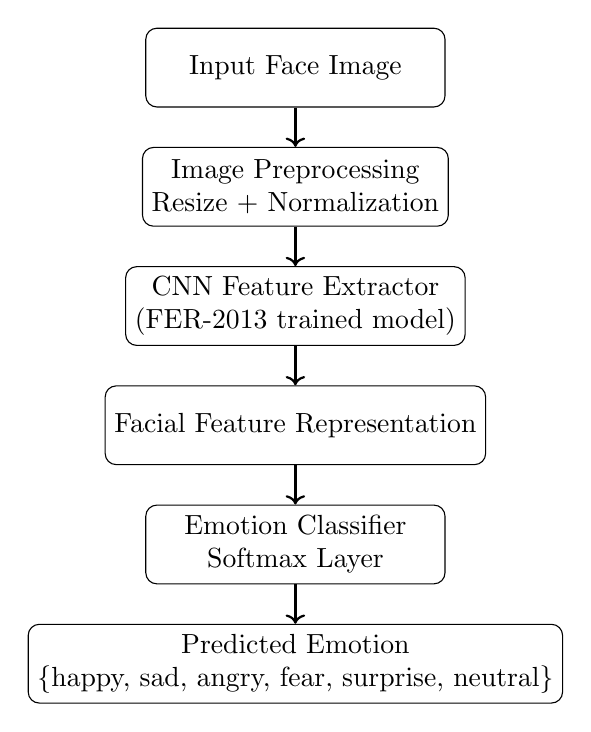
\begin{tikzpicture}[
node distance=0.5cm,
box/.style={draw, rectangle, rounded corners, align=center, minimum width=3.8cm, minimum height=1cm},
arrow/.style={->, thick}
]

\node[box] (input)
{Input Face Image};

\node[box, below=of input] (preprocess)
{Image Preprocessing\\
Resize + Normalization};

\node[box, below=of preprocess] (cnn)
{CNN Feature Extractor\\
(FER-2013 trained model)};

\node[box, below=of cnn] (features)
{Facial Feature Representation};

\node[box, below=of features] (classifier)
{Emotion Classifier\\
Softmax Layer};

\node[box, below=of classifier] (emotion)
{Predicted Emotion\\
\{happy, sad, angry, fear, surprise, neutral\}};

\draw[arrow] (input) -- (preprocess);
\draw[arrow] (preprocess) -- (cnn);
\draw[arrow] (cnn) -- (features);
\draw[arrow] (features) -- (classifier);
\draw[arrow] (classifier) -- (emotion);

\end{tikzpicture}

\end{document}